\chapter{LƯA CHỌN PHƯƠNG ÁN}
    \section{Lựa chọn nguyên lý cơ khí}
        \subsection{So sánh các kết cấu cơ khí}
            \hspace*{0.6cm}Yêu cầu:
            \begin{itemize}
                \item Đảm bảo độ bám đường, khó lật khi vào cua với tốc độ cao.
                \item Thuật toán điều khiển đơn giản.
                \item Kết cấu cơ khí vững, nhỏ gọn, ổn định và dễ chế tạo.
                \item Chủ động trong việc chuyển hướng, chuyển hướng tốt. 
            \end{itemize}
        \subsection{So sánh các sơ đồ nguyên lý}
            \hspace*{0.6cm}Xét theo từng sơ đồ nguyên lý đã tìm hiểu trong phần tổng quan, bảng dưới đây 
trình bày ưu và nhược điểm của từng loại sơ đồ:
            \begin{longtable}{|p{4cm}|p{5cm}|p{5cm}|}
                \caption{So sánh các sơ đồ nguyên lý robot} 
                \label{tab:compare_robot_schemes} \\ 
                \hline
                \textbf{Sơ đồ nguyên lý} & \textbf{Ưu điểm} & \textbf{Nhược điểm} \\
                \hline
                \endfirsthead
                \hline
                \textbf{Sơ đồ nguyên lý} & \textbf{Ưu điểm} & \textbf{Nhược điểm} \\
                \hline
                \endhead
                \hline
                \endfoot
                \hline
                \endlastfoot
                Robot Chariot \newline
                \textit{Phương án 1} \newline
                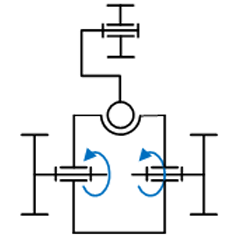
\includegraphics[width=2.5cm]{pictures/robot_chariot.png} & 
                - Kết cấu 3 bánh nhỏ gọn, đơn giản \newline
                - Mô hình toán đơn giản, dễ điều khiển & 
                - Khi vào cua dễ bị lật. \newline
                - Khả năng bám đường kém. \newline
                - Cần đảm bảo đúng trục giữa 2 bánh chủ động. \\
                \hline
                Robot SWD \newline
                \textit{Phương án 2} \newline
                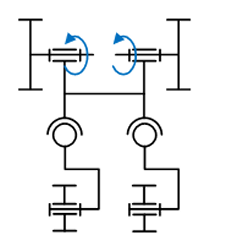
\includegraphics[width=2.5cm]{pictures/robot_swd.png} & 
                - Hai bánh chủ động phía trước kéo tải nên khó lật. \newline
                - Khả năng cân bằng tốt \newline
                - Độ ổn định khi chuyển hướng tốt & 
                - Khả năng bám đường không tốt, vào cua ở tốc độ cao dễ bị trượt. \newline
                - Mô hình tính toán phức tạp, khó điều khiển. \\
                \hline
                Robot Usain Bolt 2.0 \newline
                \textit{Phương án 3} \newline
                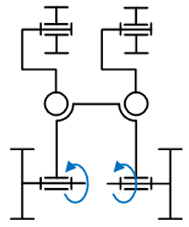
\includegraphics[width=2.5cm]{pictures/robot_usain.png} & 
                - Kết cấu 4 bánh giúp tăng khả năng tải. \newline
                - Khả năng vào cua và bám đường tốt. \newline
                - Kết cấu cơ khí đơn giản & 
                - Đảm bảo đồng trục 2 bánh dẫn động. \newline
                - Đảm bảo đồng phẳng giữa các bánh xe. \newline
                - Bị hóc đầu nếu đặt tải lệch về phía sau. \newline
                - Dễ bị lật khi vào cua với tốc độ cao. \newline
                - Mô hình tính toán phức tạp, khó điều khiển. \\
                \hline
                Robot Khepera IV \newline
                \textit{Phương án 4} \newline
                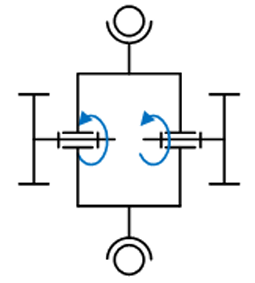
\includegraphics[width=2.5cm]{pictures/robot_khepera_IV.png} &
                - Kết cấu 4 bánh đơn giản, mô hình toán đơn giản, dễ điều khiển.\newline 
                - Trọng tâm nằm ngay trục dẫn động giữ kết cấu dễ ổn định. &
                - Khả năng vào cua kém. \newline
                - Đảm bảo đồng trục giữa 2 bánh dẫn động và đồng phẳng giữa các bánh. \newline
                - Hai bánh giữa chịu áp lực lớn vừa chịu tải vừa kéo tải. \\
                \hline
                Robot FireBall \newline
                \textit{Phương án 5} \newline
                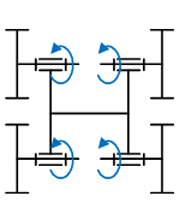
\includegraphics[width=2.5cm]{pictures/robot_fireball.png} &
                - Kết cấu cơ khí đơn giản, cân bằng tốt. \newline
                - Tải chia đều cho 4 động cơ -> giảm tải. \newline
                - Điều khiển tùy ý dễ dàng. &
                - Đảm bảo đồng trục cả 2 bánh trước và 2 bánh sau. \newline
                - Đảm bảo đồng phẳng giữa các bánh. \newline
                - Mô hình tính toán phức tạp, khó điều khiển. \\ 
            \end{longtable}
            \hspace*{0.6cm}Qua bảng so sánh trên, ta thấy phương án 3 là phương án tối ưu nhất, đáp ứng được